\hypertarget{goux6d4bux8bd5ux5de5ux5177}{%
\section{go测试工具}\label{goux6d4bux8bd5ux5de5ux5177}}

测试是go的一个子命令

\begin{Shaded}
\begin{Highlighting}[]
\ExtensionTok{go}\NormalTok{ test }\CommentTok{## go run}
\end{Highlighting}
\end{Shaded}

一个go的test文件主要文件名为 "*\textsubscript{test}.go",
它可以包含三种函数

\begin{enumerate}
\tightlist
\item
  以Test为开头的函数 测试要么,通过不通过。
\item
  以Benchmark开头的函数 会产生一个运行时间统计
\item
  以Example开头的函数 是一个样例展示函数
\end{enumerate}

*go test的机制是去搜索
"\textbf{\textsubscript{test}.go"的文件,并用一个临时main函数包裹它并运行里面测试函数。}

\hypertarget{ux6d4bux8bd5ux51fdux6570}{%
\section{测试函数}\label{ux6d4bux8bd5ux51fdux6570}}

\hypertarget{ux6d4bux8bd5ux51fdux6570-1}{%
\subsection{测试函数}\label{ux6d4bux8bd5ux51fdux6570-1}}

先来看看简单的示例。

注意:测试函数必须以Test开始

\begin{Shaded}
\begin{Highlighting}[]
\KeywordTok{func}\NormalTok{ TestName(t *testing.T) \{ }\CommentTok{// ...}
\NormalTok{\}}
\end{Highlighting}
\end{Shaded}

先来看个例子,回文的例子word.go

\begin{Shaded}
\begin{Highlighting}[]
\KeywordTok{package}\NormalTok{ word}
\KeywordTok{func}\NormalTok{ IsPalindrome(s }\DataTypeTok{string}\NormalTok{) }\DataTypeTok{bool}\NormalTok{ \{}
  \KeywordTok{for}\NormalTok{ i := }\KeywordTok{range}\NormalTok{ s \{}
    \KeywordTok{if}\NormalTok{ s[i] != s[}\BuiltInTok{len}\NormalTok{(s)-}\DecValTok{1}\NormalTok{-i] \{}
      \KeywordTok{return} \OtherTok{false}
\NormalTok{    \}}
\NormalTok{  \}}
  \KeywordTok{return} \OtherTok{true}
\NormalTok{\}}
\end{Highlighting}
\end{Shaded}

我们如何来测试这个回文函数?,创建一个word\textsubscript{test}.go

\begin{Shaded}
\begin{Highlighting}[]
\KeywordTok{package}\NormalTok{ word}
\KeywordTok{import} \StringTok{"testing"}
\KeywordTok{func}\NormalTok{ TestPalindrome(t *testing.T) \{}
  \KeywordTok{if}\NormalTok{ !IsPalindrome(}\StringTok{"detartrated"}\NormalTok{) \{}
\NormalTok{    t.Error(}\StringTok{`IsPalindrome("detartrated") = false`}\NormalTok{)}
\NormalTok{  \}}
  \KeywordTok{if}\NormalTok{ !IsPalindrome(}\StringTok{"kayak"}\NormalTok{) \{}
\NormalTok{    t.Error(}\StringTok{`IsPalindrome("kayak") = false`}\NormalTok{)}
\NormalTok{  \} \}}
\KeywordTok{func}\NormalTok{ TestNonPalindrome(t *testing.T) \{}
  \KeywordTok{if}\NormalTok{ IsPalindrome(}\StringTok{"palindrome"}\NormalTok{) \{}
\NormalTok{    t.Error(}\StringTok{`IsPalindrome("palindrome") = true`}\NormalTok{)}
\NormalTok{  \}}
\NormalTok{\}}
\end{Highlighting}
\end{Shaded}

如果正确会是如下

\begin{Shaded}
\begin{Highlighting}[]
\NormalTok{$ }\ExtensionTok{go}\NormalTok{ test}
\ExtensionTok{ok}\NormalTok{   gopl.io/ch11/word1  0.008s}
\end{Highlighting}
\end{Shaded}

错误是如下

\begin{Shaded}
\begin{Highlighting}[]
\NormalTok{$ }\KeywordTok{go}\NormalTok{ test}
\NormalTok{--- FAIL: TestFrenchPalindrome (}\DecValTok{0}\FloatTok{.00}\NormalTok{s)}
\NormalTok{word_test.}\KeywordTok{go}\NormalTok{:}\DecValTok{28}\NormalTok{: IsPalindrome(}\StringTok{"été"}\NormalTok{) = }\OtherTok{false}
\NormalTok{--- FAIL: TestCanalPalindrome (}\DecValTok{0}\FloatTok{.00}\NormalTok{s)}
\NormalTok{word_test.}\KeywordTok{go}\NormalTok{:}\DecValTok{35}\NormalTok{: IsPalindrome(}\StringTok{"A man, a plan, a canal: Panama"}\NormalTok{) = }\OtherTok{false}
\NormalTok{FAIL}
\NormalTok{FAIL    gopl.io/ch11/word1  }\DecValTok{0}\FloatTok{.014}\NormalTok{s}
\end{Highlighting}
\end{Shaded}

可以输出更为详细的信息(verbose)

\begin{Shaded}
\begin{Highlighting}[]
\NormalTok{$ }\ExtensionTok{go}\NormalTok{ test -v}
\end{Highlighting}
\end{Shaded}

用正则表达式运行其中一部分函数

\begin{Shaded}
\begin{Highlighting}[]
\NormalTok{$ }\ExtensionTok{go}\NormalTok{ test -v -run=}\StringTok{"French|Canal"}
\end{Highlighting}
\end{Shaded}

把测试用例放到一个表里面挨个测试

\begin{Shaded}
\begin{Highlighting}[]
\KeywordTok{func}\NormalTok{ TestIsPalindrome(t *testing.T) \{}
  \KeywordTok{var}\NormalTok{ tests = []}\KeywordTok{struct}\NormalTok{ \{}
\NormalTok{    input }\DataTypeTok{string}
\NormalTok{    want }\DataTypeTok{bool}
\NormalTok{  \}\{}
\NormalTok{    \{}\StringTok{""}\NormalTok{, }\OtherTok{true}\NormalTok{\},}
\NormalTok{    \{}\StringTok{"a"}\NormalTok{, }\OtherTok{true}\NormalTok{\},}
\NormalTok{    \{}\StringTok{"aa"}\NormalTok{, }\OtherTok{true}\NormalTok{\},}
\NormalTok{    \{}\StringTok{"ab"}\NormalTok{, }\OtherTok{false}\NormalTok{\},}
\NormalTok{    \{}\StringTok{"kayak"}\NormalTok{, }\OtherTok{true}\NormalTok{\},}
\NormalTok{    \{}\StringTok{"detartrated"}\NormalTok{, }\OtherTok{true}\NormalTok{\},}
\NormalTok{    \{}\StringTok{"A man, a plan, a canal: Panama"}\NormalTok{, }\OtherTok{true}\NormalTok{\},}
\NormalTok{    \{}\StringTok{"Evil I did dwell; lewd did I live."}\NormalTok{, }\OtherTok{true}\NormalTok{\},}
\NormalTok{    \{}\StringTok{"Able was I ere I saw Elba"}\NormalTok{, }\OtherTok{true}\NormalTok{\},}
\NormalTok{    \{}\StringTok{"été"}\NormalTok{, }\OtherTok{true}\NormalTok{\},}
\NormalTok{    \{}\StringTok{"Et se resservir, ivresse reste."}\NormalTok{, }\OtherTok{true}\NormalTok{\},}
\NormalTok{    \{}\StringTok{"palindrome"}\NormalTok{, }\OtherTok{false}\NormalTok{\}, }\CommentTok{// non-palindrome}
\NormalTok{    \{}\StringTok{"desserts"}\NormalTok{, }\OtherTok{false}\NormalTok{\},   }\CommentTok{// semi-palindrome}
\NormalTok{  \}}
  \KeywordTok{for}\NormalTok{ _, test := }\KeywordTok{range}\NormalTok{ tests \{}
    \KeywordTok{if}\NormalTok{ got := IsPalindrome(test.input); got != test.want \{}
\NormalTok{      t.Errorf(}\StringTok{"IsPalindrome(%q) = %v"}\NormalTok{, test.input, got)}
\NormalTok{    \}}
\NormalTok{  \}}
\NormalTok{\}}
\end{Highlighting}
\end{Shaded}

注意:

\begin{enumerate}
\tightlist
\item
  如果测试t.Errorf并不会引发panic所以如果你想中断,自己写t.Fatalf来做。
\item
  测试t.Errorf应尽量输出有用的信息
\end{enumerate}

\hypertarget{ux968fux673aux6d4bux8bd5}{%
\subsection{随机测试}\label{ux968fux673aux6d4bux8bd5}}

随机函数要注意保留该有的随机种子。方便问题复现

\hypertarget{ux7528ux4e00ux4e2aux66f4ux4e3aux6e05ux6670ux7b80ux5355ux4f46ux662fux6b63ux786eux7684ux65b9ux6cd5ux5b9eux73b0ux529fux80fd}{%
\subsubsection{用一个更为清晰简单但是正确的方法实现功能}\label{ux7528ux4e00ux4e2aux66f4ux4e3aux6e05ux6670ux7b80ux5355ux4f46ux662fux6b63ux786eux7684ux65b9ux6cd5ux5b9eux73b0ux529fux80fd}}

\hypertarget{ux5199ux4e00ux4e2aux51fdux6570ux8fd8ux4ea7ux751fux6d4bux8bd5ux6570ux636e}{%
\subsubsection{写一个函数还产生测试数据}\label{ux5199ux4e00ux4e2aux51fdux6570ux8fd8ux4ea7ux751fux6d4bux8bd5ux6570ux636e}}

gen-\textgreater{}{[}(test\textsubscript{1},result\textsubscript{1}),(test\textsubscript{2},result\textsubscript{2}{]},(test\textsubscript{3},
result\textsubscript{3}),\ldots{},(test\textsubscript{n},result\textsubscript{n}))

\begin{Shaded}
\begin{Highlighting}[]
\CommentTok{//!+random}
\CommentTok{// randomPalindrome returns a palindrome whose length and contents}
\CommentTok{// are derived from the pseudo-random number generator rng.}
\KeywordTok{func}\NormalTok{ randomPalindrome(rng *rand.Rand) }\DataTypeTok{string}\NormalTok{ \{}
\NormalTok{  n := rng.Intn(}\DecValTok{25}\NormalTok{) }\CommentTok{// random length up to 24}
\NormalTok{  runes := }\BuiltInTok{make}\NormalTok{([]}\DataTypeTok{rune}\NormalTok{, n)}
  \KeywordTok{for}\NormalTok{ i := }\DecValTok{0}\NormalTok{; i < (n+}\DecValTok{1}\NormalTok{)/}\DecValTok{2}\NormalTok{; i++ \{}
\NormalTok{    r := }\DataTypeTok{rune}\NormalTok{(rng.Intn(}\DecValTok{0x1000}\NormalTok{)) }\CommentTok{// random rune up to '\textbackslash{}u0999'}
\NormalTok{    runes[i] = r}
\NormalTok{    runes[n}\DecValTok{-1}\NormalTok{-i] = r}
\NormalTok{  \}}
  \KeywordTok{return} \DataTypeTok{string}\NormalTok{(runes)}
\NormalTok{\}}

\KeywordTok{func}\NormalTok{ TestRandomPalindromes(t *testing.T) \{}
  \CommentTok{// Initialize a pseudo-random number generator.}
\NormalTok{  seed := time.Now().UTC().UnixNano()}
\NormalTok{  t.Logf(}\StringTok{"Random seed: %d"}\NormalTok{, seed)}
\NormalTok{  rng := rand.New(rand.NewSource(seed))}

  \KeywordTok{for}\NormalTok{ i := }\DecValTok{0}\NormalTok{; i < }\DecValTok{1000}\NormalTok{; i++ \{}
\NormalTok{    p := randomPalindrome(rng)}
    \KeywordTok{if}\NormalTok{ !IsPalindrome(p) \{}
\NormalTok{      t.Errorf(}\StringTok{"IsPalindrome(%q) = false"}\NormalTok{, p)}
\NormalTok{    \}}
\NormalTok{  \}}
\NormalTok{\}}
\end{Highlighting}
\end{Shaded}

\hypertarget{ux6d4bux8bd5ux547dux4ee4ux8fd0ux7528ux4e86ux767dux76d2ux6d4bux8bd5}{%
\subsection{测试命令(运用了白盒测试)}\label{ux6d4bux8bd5ux547dux4ee4ux8fd0ux7528ux4e86ux767dux76d2ux6d4bux8bd5}}

测试带命令行的程序

\hypertarget{ux547dux4ee4ux884cux51fdux6570}{%
\subsubsection{命令行函数}\label{ux547dux4ee4ux884cux51fdux6570}}

\begin{Shaded}
\begin{Highlighting}[]
\KeywordTok{var}\NormalTok{ (}
\NormalTok{  n = flag.Bool(}\StringTok{"n"}\NormalTok{, }\OtherTok{false}\NormalTok{, }\StringTok{"omit trailing newline"}\NormalTok{)}
\NormalTok{  s = flag.String(}\StringTok{"s"}\NormalTok{, }\StringTok{" "}\NormalTok{, }\StringTok{"separator"}\NormalTok{)}
\NormalTok{)}

\KeywordTok{var}\NormalTok{ out io.Writer = os.Stdout }\CommentTok{// modified during testing}

\KeywordTok{func}\NormalTok{ main() \{}
\NormalTok{  flag.Parse()}
  \KeywordTok{if}\NormalTok{ err := echo(!*n, *s, flag.Args()); err != }\OtherTok{nil}\NormalTok{ \{}
\NormalTok{    fmt.Fprintf(os.Stderr, }\StringTok{"echo: %v}\CharTok{\textbackslash{}n}\StringTok{"}\NormalTok{, err)}
\NormalTok{    os.Exit(}\DecValTok{1}\NormalTok{)}
\NormalTok{  \}}
\NormalTok{\}}

\KeywordTok{func}\NormalTok{ echo(newline }\DataTypeTok{bool}\NormalTok{, sep }\DataTypeTok{string}\NormalTok{, args []}\DataTypeTok{string}\NormalTok{) }\DataTypeTok{error}\NormalTok{ \{}
\NormalTok{  fmt.Fprint(out, strings.Join(args, sep))}
  \KeywordTok{if}\NormalTok{ newline \{}
\NormalTok{    fmt.Fprintln(out)}
\NormalTok{  \}}
  \KeywordTok{return} \OtherTok{nil}
\NormalTok{\}}
\end{Highlighting}
\end{Shaded}

如何测试这个函数?

\begin{Shaded}
\begin{Highlighting}[]
\OperatorTok{>>} \ExtensionTok{go}\NormalTok{ run echo.go -n=false -s=}\StringTok{"'"}\NormalTok{ some some some}
\OperatorTok{>>} \ExtensionTok{some}\StringTok{'some'}\NormalTok{some}
\end{Highlighting}
\end{Shaded}

\hypertarget{ux6d4bux8bd5ux4ee3ux7801}{%
\subsubsection{测试代码}\label{ux6d4bux8bd5ux4ee3ux7801}}

\begin{Shaded}
\begin{Highlighting}[]
\KeywordTok{func}\NormalTok{ TestEcho(t *testing.T) \{}
  \KeywordTok{var}\NormalTok{ tests = []}\KeywordTok{struct}\NormalTok{ \{}
\NormalTok{    newline }\DataTypeTok{bool}
\NormalTok{    sep     }\DataTypeTok{string}
\NormalTok{    args    []}\DataTypeTok{string}
\NormalTok{    want    }\DataTypeTok{string}
\NormalTok{  \}\{}
\NormalTok{    \{}\OtherTok{true}\NormalTok{, }\StringTok{""}\NormalTok{, []}\DataTypeTok{string}\NormalTok{\{\}, }\StringTok{"}\CharTok{\textbackslash{}n}\StringTok{"}\NormalTok{\},}
\NormalTok{    \{}\OtherTok{false}\NormalTok{, }\StringTok{""}\NormalTok{, []}\DataTypeTok{string}\NormalTok{\{\}, }\StringTok{""}\NormalTok{\},}
\NormalTok{    \{}\OtherTok{true}\NormalTok{, }\StringTok{"}\CharTok{\textbackslash{}t}\StringTok{"}\NormalTok{, []}\DataTypeTok{string}\NormalTok{\{}\StringTok{"one"}\NormalTok{, }\StringTok{"two"}\NormalTok{, }\StringTok{"three"}\NormalTok{\}, }\StringTok{"one}\CharTok{\textbackslash{}t}\StringTok{two}\CharTok{\textbackslash{}t}\StringTok{three}\CharTok{\textbackslash{}n}\StringTok{"}\NormalTok{\},}
\NormalTok{    \{}\OtherTok{true}\NormalTok{, }\StringTok{","}\NormalTok{, []}\DataTypeTok{string}\NormalTok{\{}\StringTok{"a"}\NormalTok{, }\StringTok{"b"}\NormalTok{, }\StringTok{"c"}\NormalTok{\}, }\StringTok{"a,b,c}\CharTok{\textbackslash{}n}\StringTok{"}\NormalTok{\},}
\NormalTok{    \{}\OtherTok{false}\NormalTok{, }\StringTok{":"}\NormalTok{, []}\DataTypeTok{string}\NormalTok{\{}\StringTok{"1"}\NormalTok{, }\StringTok{"2"}\NormalTok{, }\StringTok{"3"}\NormalTok{\}, }\StringTok{"1:2:3"}\NormalTok{\},}
\NormalTok{  \}}

  \KeywordTok{for}\NormalTok{ _, test := }\KeywordTok{range}\NormalTok{ tests \{}
\NormalTok{    descr := fmt.Sprintf(}\StringTok{"echo(%v, %q, %q)"}\NormalTok{,}
\NormalTok{      test.newline, test.sep, test.args)}

\NormalTok{    out = }\BuiltInTok{new}\NormalTok{(bytes.Buffer) }\CommentTok{// captured output 这里修改了包体变量out原本为stdout现在为一个buffer}
    \KeywordTok{if}\NormalTok{ err := echo(test.newline, test.sep, test.args); err != }\OtherTok{nil}\NormalTok{ \{}
\NormalTok{      t.Errorf(}\StringTok{"%s failed: %v"}\NormalTok{, descr, err)}
      \KeywordTok{continue}
\NormalTok{    \}}
\NormalTok{    got := out.(*bytes.Buffer).String()}
    \KeywordTok{if}\NormalTok{ got != test.want \{}
\NormalTok{      t.Errorf(}\StringTok{"%s = %q, want %q"}\NormalTok{, descr, got, test.want)}
\NormalTok{    \}}
\NormalTok{  \}}
\NormalTok{\}}
\end{Highlighting}
\end{Shaded}

NOTE:

\begin{enumerate}
\tightlist
\item
  在测试的代码里面不要调用 log.Fatal 或者
  os.Exit,因为这两个调用会阻止跟踪的过程,这两个函数的调用可以认为是main函数的特权
  。
\end{enumerate}

\hypertarget{ux767dux76d2ux6d4bux8bd5}{%
\subsection{白盒测试}\label{ux767dux76d2ux6d4bux8bd5}}

\begin{enumerate}
\tightlist
\item
  回文测试是黑盒测试
\item
  echo测试是白盒测试(因为我们修改echo的变量out,所以实际上我们是知道echo程序的代码结构的)
\end{enumerate}

\hypertarget{ux90aeux4ef6ux7a7aux95f4ux9884ux8b66}{%
\subsubsection{邮件空间预警}\label{ux90aeux4ef6ux7a7aux95f4ux9884ux8b66}}

\begin{Shaded}
\begin{Highlighting}[]
\KeywordTok{var}\NormalTok{ usage = }\BuiltInTok{make}\NormalTok{(}\KeywordTok{map}\NormalTok{[}\DataTypeTok{string}\NormalTok{]}\DataTypeTok{int64}\NormalTok{)}

\KeywordTok{func}\NormalTok{ bytesInUse(username }\DataTypeTok{string}\NormalTok{) }\DataTypeTok{int64}\NormalTok{ \{ }\KeywordTok{return}\NormalTok{ usage[username] \}}

\CommentTok{// Email sender configuration.}
\CommentTok{// }\AlertTok{NOTE}\CommentTok{: never put passwords in source code!}
\KeywordTok{const}\NormalTok{ sender = }\StringTok{"notifications@example.com"}
\KeywordTok{const}\NormalTok{ password = }\StringTok{"correcthorsebatterystaple"}
\KeywordTok{const}\NormalTok{ hostname = }\StringTok{"smtp.example.com"}

\KeywordTok{const}\NormalTok{ template = }\StringTok{`Warning: you are using %d bytes of storage,}
\StringTok{%d%% of your quota.`}

\KeywordTok{func}\NormalTok{ CheckQuota(username }\DataTypeTok{string}\NormalTok{) \{}
\NormalTok{  used := bytesInUse(username)}
  \KeywordTok{const}\NormalTok{ quota = }\DecValTok{1000000000} \CommentTok{// 1GB}
\NormalTok{  percent := }\DecValTok{100}\NormalTok{ * used / quota}
  \KeywordTok{if}\NormalTok{ percent < }\DecValTok{90}\NormalTok{ \{}
    \KeywordTok{return} \CommentTok{// OK}
\NormalTok{  \}}
\NormalTok{  msg := fmt.Sprintf(template, used, percent)}
\NormalTok{  auth := smtp.PlainAuth(}\StringTok{""}\NormalTok{, sender, password, hostname)}
\NormalTok{  err := smtp.SendMail(hostname+}\StringTok{":587"}\NormalTok{, auth, sender,}
\NormalTok{    []}\DataTypeTok{string}\NormalTok{\{username\}, []}\DataTypeTok{byte}\NormalTok{(msg))}
  \KeywordTok{if}\NormalTok{ err != }\OtherTok{nil}\NormalTok{ \{}
\NormalTok{    log.Printf(}\StringTok{"smtp.SendMail(%s) failed: %s"}\NormalTok{, username, err)}
\NormalTok{  \}}
\NormalTok{\}}

\end{Highlighting}
\end{Shaded}

函数功能:当用户的使用空间炒股90percent的时候,发送一封邮件给用户。

为了测试这个功能是否正确。我们改变源码。把notifyUser抽象出来做一个发送邮件的函数

\begin{Shaded}
\begin{Highlighting}[]
\KeywordTok{var}\NormalTok{ usage = }\BuiltInTok{make}\NormalTok{(}\KeywordTok{map}\NormalTok{[}\DataTypeTok{string}\NormalTok{]}\DataTypeTok{int64}\NormalTok{)}

\KeywordTok{func}\NormalTok{ bytesInUse(username }\DataTypeTok{string}\NormalTok{) }\DataTypeTok{int64}\NormalTok{ \{ }\KeywordTok{return}\NormalTok{ usage[username] \}}

\CommentTok{// E-mail sender configuration.}
\CommentTok{// }\AlertTok{NOTE}\CommentTok{: never put passwords in source code!}
\KeywordTok{const}\NormalTok{ sender = }\StringTok{"notifications@example.com"}
\KeywordTok{const}\NormalTok{ password = }\StringTok{"correcthorsebatterystaple"}
\KeywordTok{const}\NormalTok{ hostname = }\StringTok{"smtp.example.com"}

\KeywordTok{const}\NormalTok{ template = }\StringTok{`Warning: you are using %d bytes of storage,}
\StringTok{%d%% of your quota.`}

\CommentTok{//!+factored}
\KeywordTok{var}\NormalTok{ notifyUser = }\KeywordTok{func}\NormalTok{(username, msg }\DataTypeTok{string}\NormalTok{) \{}
\NormalTok{  auth := smtp.PlainAuth(}\StringTok{""}\NormalTok{, sender, password, hostname)}
\NormalTok{  err := smtp.SendMail(hostname+}\StringTok{":587"}\NormalTok{, auth, sender,}
\NormalTok{    []}\DataTypeTok{string}\NormalTok{\{username\}, []}\DataTypeTok{byte}\NormalTok{(msg))}
  \KeywordTok{if}\NormalTok{ err != }\OtherTok{nil}\NormalTok{ \{}
\NormalTok{    log.Printf(}\StringTok{"smtp.SendMail(%s) failed: %s"}\NormalTok{, username, err)}
\NormalTok{  \}}
\NormalTok{\}}

\KeywordTok{func}\NormalTok{ CheckQuota(username }\DataTypeTok{string}\NormalTok{) \{}
\NormalTok{  used := bytesInUse(username)}
  \KeywordTok{const}\NormalTok{ quota = }\DecValTok{1000000000} \CommentTok{// 1GB}
\NormalTok{  percent := }\DecValTok{100}\NormalTok{ * used / quota}
  \KeywordTok{if}\NormalTok{ percent < }\DecValTok{90}\NormalTok{ \{}
    \KeywordTok{return} \CommentTok{// OK}
\NormalTok{  \}}
\NormalTok{  msg := fmt.Sprintf(template, used, percent)}
\NormalTok{  notifyUser(username, msg)}
\NormalTok{\}}
\end{Highlighting}
\end{Shaded}

测试90功能是否正确,替换掉原来的notifyUser,不做实际发送操作。

\begin{Shaded}
\begin{Highlighting}[]
\KeywordTok{func}\NormalTok{ TestCheckQuotaNotifiesUser(t *testing.T) \{}
  \KeywordTok{var}\NormalTok{ notifiedUser, notifiedMsg }\DataTypeTok{string}
\NormalTok{  notifyUser = }\KeywordTok{func}\NormalTok{(user, msg }\DataTypeTok{string}\NormalTok{) \{}
\NormalTok{    notifiedUser, notifiedMsg = user, msg}
\NormalTok{  \}}

  \KeywordTok{const}\NormalTok{ user = }\StringTok{"joe@example.org"}
\NormalTok{  usage[user] = }\DecValTok{980000000} \CommentTok{// simulate a 980MB-used condition}

\NormalTok{  CheckQuota(user)}
  \KeywordTok{if}\NormalTok{ notifiedUser == }\StringTok{""}\NormalTok{ && notifiedMsg == }\StringTok{""}\NormalTok{ \{}
\NormalTok{    t.Fatalf(}\StringTok{"notifyUser not called"}\NormalTok{)}
\NormalTok{  \}}
  \KeywordTok{if}\NormalTok{ notifiedUser != user \{}
\NormalTok{    t.Errorf(}\StringTok{"wrong user (%s) notified, want %s"}\NormalTok{,}
\NormalTok{      notifiedUser, user)}
\NormalTok{  \}}
  \KeywordTok{const}\NormalTok{ wantSubstring = }\StringTok{"98% of your quota"}
  \KeywordTok{if}\NormalTok{ !strings.Contains(notifiedMsg, wantSubstring) \{}
\NormalTok{    t.Errorf(}\StringTok{"unexpected notification message <<%s>>, "}\NormalTok{+}
      \StringTok{"want substring %q"}\NormalTok{, notifiedMsg, wantSubstring)}
\NormalTok{  \}}
\NormalTok{\}}

\CommentTok{//!-test}
\end{Highlighting}
\end{Shaded}

恢复现场

\begin{Shaded}
\begin{Highlighting}[]
\KeywordTok{func}\NormalTok{ TestCheckQuotaNotifiesUser(t *testing.T) \{}
  \CommentTok{// Save and restore original notifyUser.}
\NormalTok{  saved := notifyUser}
  \KeywordTok{defer} \KeywordTok{func}\NormalTok{() \{ notifyUser = saved \}()}

  \CommentTok{// Install the test's fake notifyUser.}
  \KeywordTok{var}\NormalTok{ notifiedUser, notifiedMsg }\DataTypeTok{string}
\NormalTok{  notifyUser = }\KeywordTok{func}\NormalTok{(user, msg }\DataTypeTok{string}\NormalTok{) \{}
\NormalTok{    notifiedUser, notifiedMsg = user, msg}
\NormalTok{  \}}
  \CommentTok{// ...rest of test...}
\NormalTok{\}}
\end{Highlighting}
\end{Shaded}

\hypertarget{ux603bux7ed3ux4e00ux4e0bux767dux76d2ux6d4bux8bd5ux7684ux8fc7ux7a0b}{%
\subsubsection{总结一下白盒测试的过程}\label{ux603bux7ed3ux4e00ux4e0bux767dux76d2ux6d4bux8bd5ux7684ux8fc7ux7a0b}}

\begin{enumerate}
\tightlist
\item
  替换掉原本的函数
\item
  测试
\item
  回复现场
\end{enumerate}

\hypertarget{ux5916ux90e8ux6d4bux8bd5ux5305}{%
\subsection{外部测试包}\label{ux5916ux90e8ux6d4bux8bd5ux5305}}

\textbf{有一个url的测试函数需要用到http。那么需要在net/url包中声明这个测试函数会导致包循环引用,如图中向上的箭头所示,但是10.1节讲过,
Go规范禁止循环引用.}

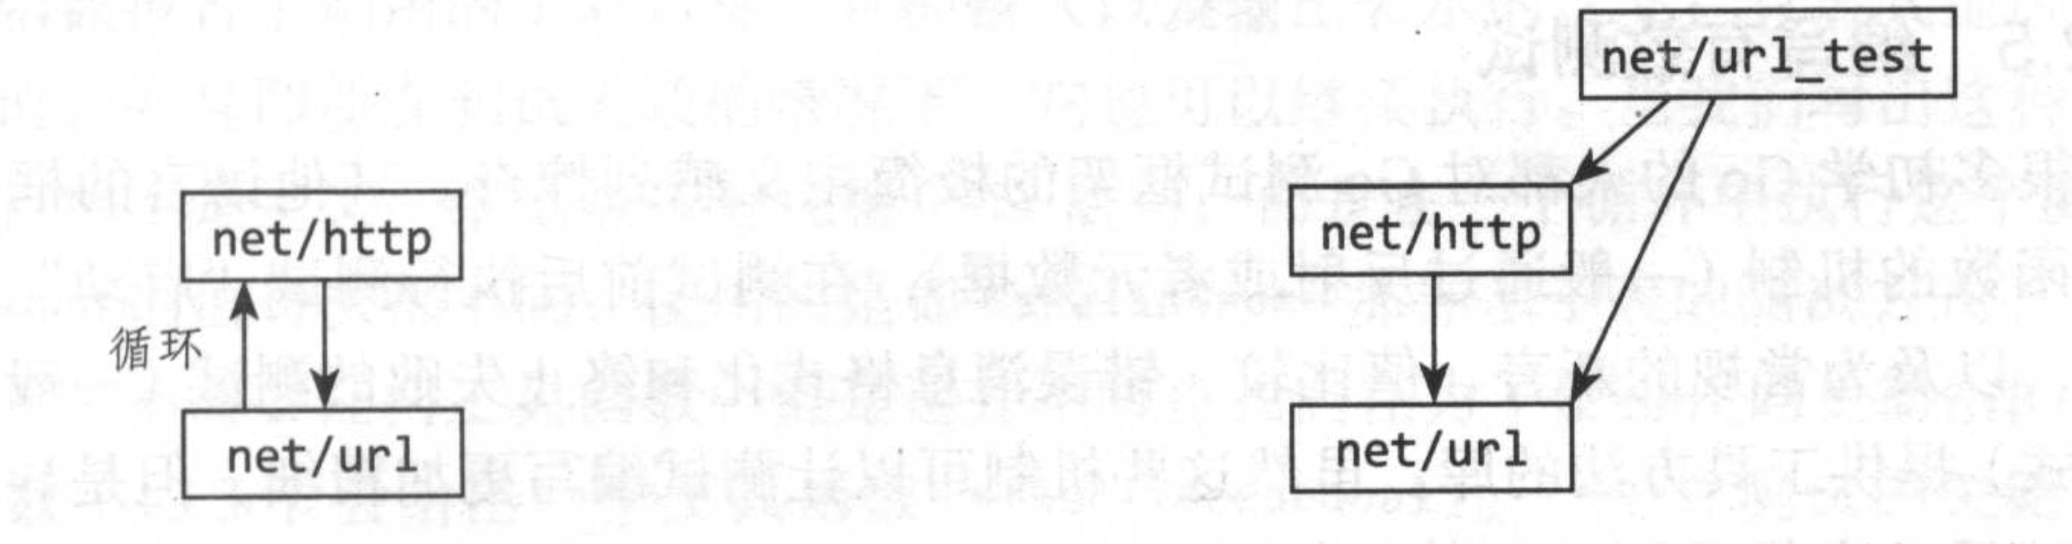
\includegraphics{./ch11/xunhuan.png}

\hypertarget{ux5305ux5185ux6d4bux8bd5}{%
\subsubsection{包内测试}\label{ux5305ux5185ux6d4bux8bd5}}

和代码写相同的包名

\hypertarget{ux5305ux5916ux6d4bux8bd5}{%
\subsubsection{包外测试}\label{ux5305ux5916ux6d4bux8bd5}}

比如写

\begin{Shaded}
\begin{Highlighting}[]
\KeywordTok{package}\NormalTok{ url_test }\CommentTok{//和url不是一个包,但是可以引入url和http包来测试url包}
\end{Highlighting}
\end{Shaded}

\hypertarget{ux5982ux4f55ux5224ux65adux4e00ux4e2aux5305ux7684ux6587ux4ef6ux79cdux7c7b}{%
\subsubsection{如何判断一个包的文件种类}\label{ux5982ux4f55ux5224ux65adux4e00ux4e2aux5305ux7684ux6587ux4ef6ux79cdux7c7b}}

\begin{enumerate}
\item
  一般文件

\begin{Shaded}
\begin{Highlighting}[]
\NormalTok{$ }\ExtensionTok{go}\NormalTok{ list -f=}\DataTypeTok{\{\{.GoFiles\}\}}\NormalTok{ fmt}
\NormalTok{[}\ExtensionTok{doc.go}\NormalTok{ format.go print.go scan.go]}
\end{Highlighting}
\end{Shaded}
\item
  包内测试文件

\begin{Shaded}
\begin{Highlighting}[]
\NormalTok{$ }\ExtensionTok{go}\NormalTok{ list -f=}\DataTypeTok{\{\{.TestGoFiles\}\}}\NormalTok{ fmt}
\NormalTok{[}\ExtensionTok{export_test.go}\NormalTok{]}
\end{Highlighting}
\end{Shaded}
\item
  包外测试

\begin{Shaded}
\begin{Highlighting}[]
\NormalTok{$ }\ExtensionTok{go}\NormalTok{ list -f=}\DataTypeTok{\{\{.XTestGoFiles\}\}}\NormalTok{ fmt}
\NormalTok{[}\ExtensionTok{fmt_test.go}\NormalTok{ scan_test.go stringer_test.go]}
\end{Highlighting}
\end{Shaded}
\end{enumerate}

\hypertarget{ux5982ux4f55ux8ba9ux5305ux5916ux6d4bux8bd5ux8bbfux95eeux5230ux5305ux5185ux7684ux53d8ux91cf}{%
\subsubsection{如何让包外测试访问到包内的变量?}\label{ux5982ux4f55ux8ba9ux5305ux5916ux6d4bux8bd5ux8bbfux95eeux5230ux5305ux5185ux7684ux53d8ux91cf}}

专门写一个export\textsubscript{test}.go来暴露包内测试的变量。这样外部测试包就可以访问包内的变量了。

\hypertarget{ux7f16ux5199ux6709ux6548ux6d4bux8bd5}{%
\subsection{编写有效测试}\label{ux7f16ux5199ux6709ux6548ux6d4bux8bd5}}

\begin{enumerate}
\tightlist
\item
  go的测试非常简单,go的逻辑是,让写代码的人来维护代码。所以代码和测试代码差不多。
\item
  不要在测试里面panic,这样是无效的测试。因为没有为维护者提供信息。
\end{enumerate}

\hypertarget{ux907fux514dux8106ux5f31ux6d4bux8bd5}{%
\subsection{避免脆弱测试}\label{ux907fux514dux8106ux5f31ux6d4bux8bd5}}

测试如果不稳定,那么程序编写人员会非常难受。

\hypertarget{ux8986ux76d6ux7387}{%
\section{覆盖率}\label{ux8986ux76d6ux7387}}

\begin{Shaded}
\begin{Highlighting}[]
\ExtensionTok{go}\NormalTok{ test -v -run=Coverage gopl.io/ch7/eval}
\ExtensionTok{go}\NormalTok{ test -run=Coverage -coverprofile=c.out gopl.io/ch7/eval}
\ExtensionTok{-covermode}\NormalTok{=count }\CommentTok{##可以显示代码被执行的次数}
\end{Highlighting}
\end{Shaded}

覆盖率不是总会百分之100执行,比如有的代码可能永远不会执行到

\hypertarget{benchmarkux51fdux6570}{%
\section{benchmark函数}\label{benchmarkux51fdux6570}}

\begin{enumerate}
\tightlist
\item
  函数名要以Benchmark开头
\item
  *testing.T作为函数参数
\end{enumerate}

\begin{Shaded}
\begin{Highlighting}[]
\KeywordTok{import} \StringTok{"testing"}
\KeywordTok{func}\NormalTok{ BenchmarkIsPalindrome(b *testing.B) \{}
  \KeywordTok{for}\NormalTok{ i := }\DecValTok{0}\NormalTok{; i < b.N; i++ \{}
\NormalTok{    IsPalindrome(}\StringTok{"A man, a plan, a canal: Panama"}\NormalTok{)}
\NormalTok{  \}}
\NormalTok{\}}
\end{Highlighting}
\end{Shaded}

\begin{Shaded}
\begin{Highlighting}[]
\ExtensionTok{go}\NormalTok{ test -bench=.}
\ExtensionTok{go}\NormalTok{ test -bench=. -benchmem }\CommentTok{##可以查看内存情况。}
\end{Highlighting}
\end{Shaded}

最后会产生报告,其中N是测试命令自己会根据程序运行情况调整大小的。最后可以从报告中看出来大小。

\hypertarget{ux6027ux80fdux5256ux6790}{%
\section{性能剖析}\label{ux6027ux80fdux5256ux6790}}

\begin{enumerate}
\tightlist
\item
  不要过早优化。
\item
  如何优化关键代码?使用工具剖析,不要使用靠自己的直觉。因为关键代码很有可能和你的直觉不一样。
\end{enumerate}

\hypertarget{ux4e09ux4e2dux6027ux80fdux5256ux6790ux5de5ux5177}{%
\subsection{三中性能剖析工具}\label{ux4e09ux4e2dux6027ux80fdux5256ux6790ux5de5ux5177}}

\begin{Shaded}
\begin{Highlighting}[]
\NormalTok{$ }\ExtensionTok{go}\NormalTok{ test -cpuprofile=cpu.out     ## cpu}
\NormalTok{$ }\ExtensionTok{go}\NormalTok{ test -blockprofile=block.out }\CommentTok{## 阻塞}
\NormalTok{$ }\ExtensionTok{go}\NormalTok{ test -memprofile=mem.out     ## 内存}
\end{Highlighting}
\end{Shaded}

\hypertarget{ux8fd0ux884cux65f6ux5185ux5b58ux5256ux6790}{%
\subsection{运行时内存剖析}\label{ux8fd0ux884cux65f6ux5185ux5b58ux5256ux6790}}

\begin{enumerate}
\tightlist
\item
  长时间运行的程序分析,无法如上面那样仅仅启动分析就行。
\item
  可以使用runtime API来启动
\end{enumerate}

\hypertarget{ux6027ux80fdux5256ux6790ux5de5ux5177}{%
\subsection{性能剖析工具}\label{ux6027ux80fdux5256ux6790ux5de5ux5177}}

如果运行时产生了数据,那么就可以用工具来分析

\begin{Shaded}
\begin{Highlighting}[]
\ExtensionTok{go}\NormalTok{ tool pprof}
\end{Highlighting}
\end{Shaded}

更过的关于性能剖析的方法,请参考阅读\href{https://blog.golang.org/profiling-go-programs}{Profiling
Go Programs}【博客】

\hypertarget{exampleux51fdux6570}{%
\section{Example函数}\label{exampleux51fdux6570}}

\begin{Shaded}
\begin{Highlighting}[]
\KeywordTok{func}\NormalTok{ ExampleIsPalindrome() \{}
\NormalTok{  fmt.Println(IsPalindrome(}\StringTok{"A man, a plan, a canal: Panama"}\NormalTok{))}
\NormalTok{  fmt.Println(IsPalindrome(}\StringTok{"palindrome"}\NormalTok{))}
  \CommentTok{// Output:}
  \CommentTok{// true}
  \CommentTok{// false}
\NormalTok{\}}

\end{Highlighting}
\end{Shaded}

\begin{enumerate}
\tightlist
\item
  示例作用
\item
  如果包含Output测试函数回去运行它,并检测输出是否一致。
\item
  展示在web-based的应用中。
\end{enumerate}
